\documentclass[12pt, a4paper]{article}
\usepackage{titlesec}
\usepackage{graphicx}
\usepackage{hyperref}
\usepackage{amsmath}
\renewcommand{\figurename}{Fig.}
\titlelabel{\thetitle.\quad}
\author{Pēteris Račinskis pr20015}
\date{19/12/21}
\begin{document}
\title{Homework 2}

\maketitle

\section{Small zero-sum simultaneous game}

Filled-in payoff matrix:
\begin{equation}
\boldsymbol{\pi}=\begin{bmatrix}
    -6 & 3 & 1 \\
    4 & -\frac{2}{3} & 2 
\end{bmatrix}
\end{equation}

\subsection{Majorant and minorant games}

In the majorant version of the game, player 2 has to go first and player 1 gets to respond. Best responses are $(1) \rightarrow 2, \pi_{21}=4$; $(2) \rightarrow 1, \pi_{12}=3$ and $(3) \rightarrow 2, \pi_{23}=2$. Consequently p2 picks (3), with the value of the game at $(2,-2)$.

In the minorant version of the game, p1 goes first and p2 gets to pick their best response for $(1) \rightarrow 1, \pi_{11}=-6$; $(2) \rightarrow 2, \pi_{22}=-\frac{2}{3}$. p1 therefore picks (2) with the value of the game at $(-\frac{2}{3}, \frac{2}{3})$.

\subsection{Simultaneous game equilibrium}

In the simultaneous version of the game, p2's strategy (3) is strictly dominated by a range of mixed strategies ($(1)q+(2)(1-q)$ with $\frac{2}{9} \leq q \leq \frac{4}{7}$), so it can be eliminated from the payoff matrix. Furthermore, there are no pure strategy Nash equilibria, and to get the indifference equation to produce a valid probability distribution, the actual (negative) utility values of p2 need to be used in it. The payoff matrices used are therefore:

\begin{equation}
    \boldsymbol{\pi^{1}}=\begin{bmatrix}
        -6 & 3 \\
        4 & -\frac{2}{3} \\ 
    \end{bmatrix}
    ;
    \boldsymbol{\pi^{2}}=\begin{bmatrix}
        6 & -3 \\
        -4 & \frac{2}{3} \\ 
    \end{bmatrix}
\end{equation}

For a mixed strategy with a given set of support strategies to be rationalizable for either player, the expected payoffs of all strategies in the support set must be equal. The equilibrium mixed strategy of p1 and p2's expected utility can therefore be found from p2's payoff matrix as follows

\begin{equation}
    6p-4(1-p) = -3p + \frac{2}{3}(1-p)
\end{equation}
\begin{equation}
    10p-4=-\frac{11}{3}p+\frac{2}{3}
\end{equation}
\begin{equation}
    -41p = 14
\end{equation}
\begin{equation}
    s_1=\frac{14}{41}(1)+\frac{27}{41}(2);E_2=-\frac{24}{41}
\end{equation}

while p2's strategy and p1's expected utility are given by

\begin{equation}
    -6q+3(1-q) = 4q - \frac{2}{3}(1-q)
\end{equation}
\begin{equation}
    -9q+3=4\frac{2}{3}q-\frac{2}{3}
\end{equation}
\begin{equation}
    -41q = 11
\end{equation}
\begin{equation}
    s_2=\frac{11}{41}(1)+\frac{30}{41}(2);E_1=\frac{24}{41}
\end{equation}

p1 is indifferent to the choice of row, whereas p2 is indifferent between the two columns in the strategy's support, while preferring both to the expected value of selecting column 3, which is $\frac{-1*14}{41}+\frac{-2*27}{41}=-\frac{68}{41}<E_2$. Thus neither player has any incentive to deviate from this equilibrium and the expected value is secured.

\section{Large zero-sum simultaneous game}

Filled-in payoff matrix:

\begin{equation}
    \boldsymbol{\pi}=\begin{bmatrix}
        0 & 5 & -1 & \frac{5}{4} \\
        0 & 0 & 7 & -6 \\
        9 & -1 & \frac{1}{8} & 13 \\ 
    \end{bmatrix}
\end{equation}

\subsection{Minorant and majorant games}

In the majorant case, p1's best responses are $(1) \rightarrow 3, \pi_{31}=(9,-9)$; $(2) \rightarrow 1, \pi_{12}=(5,-5)$; $(3) \rightarrow 2, \pi_{23}=(7,-7)$; $(4) \rightarrow 3, \pi_{34}=(13,-13)$. p2 picks (2) for a value of $(5,-5)$.

In the minorant case, p2's best responses are $(1) \rightarrow 3, \pi_{13}=(-1,1)$; $(2) \rightarrow 4, \pi_{24}=(-6,6)$; $(3) \rightarrow 2, \pi_{32}=(-1,1)$. p1 picks (1), (3) or a mixed strategy for a value of $(-1,1)$.


\subsection{Simultaneous game}

No pure equilibria exist. Thus there are two approaches that succeed at solving this game - finding the support set for p2's equilibrium mixed strategy and solving a system of equations, or converting the game into a form that can be handled by a Linear Programming algorithm.


For the first approach, which was the one I originally took, one can (successfully) guess that since column 1 is a never best response in terms of pure strategies, and looks like it might be dominated by a mixed strategy of the other columns, one could drop it and reduce the payoff matrix to

\begin{equation}
    \boldsymbol{\pi}=\begin{bmatrix}
        5 & -1 & \frac{5}{4} \\
        0 & 7 & -6 \\
        -1 & \frac{1}{8} & 13 \\ 
    \end{bmatrix}
\end{equation}

which can then be expressed as the following systems of indifference equations

\begin{equation}
    \begin{cases}
        -5p_1-0p_2+1(1-p_1-p_2)-E_2=0 \\
        1p_1-7p_2-\frac{1}{8}(1-p_1-p_2)-E_2=0 \\
        -\frac{5}{4}p_1+6p_2-13(1-p_1-p_2)-E_2=0 \\
    \end{cases}
\end{equation}
\begin{equation}
    \begin{cases}
        5q_1-1q_2+\frac{5}{4}(1-q_1-q_2)-E_1=0 \\
        0q_1+7p_2-6(1-q_1-q_2)-E_1=0 \\
        -1q_1+\frac{1}{8}q_2+13(1-q_1-q_2)-E_1=0 \\
    \end{cases}
\end{equation}

rearranged as the augmented matrices

\begin{equation}
    \begin{bmatrix}
        -6 & -1 & -1 & -1 \\
        \frac{9}{8} & -\frac{55}{8} & -1 & \frac{1}{8}\\
        \frac{47}{9} & 19 & -1 & 13 \\ 
    \end{bmatrix}
\end{equation}
\begin{equation}
    \begin{bmatrix}
        \frac{15}{4} & -\frac{9}{4} & -1 & -\frac{5}{4} \\
        6 & 13 & -1 & 6 \\
        -14 & -\frac{103}{8} & -1 & -13 \\ 
    \end{bmatrix}
\end{equation}

and solved using an algorithm like Gaussian elimination. Since working with so many numbers at once is quite error prone (at least for me), this is best left to a computer. Using a \href{https://matrixcalc.org/en/slu.html}{solver available online} the following results were obtained:

\begin{equation}
    p_1=\frac{3352}{7897};p_2=\frac{2553}{7897};p_3=\frac{1992}{7897};E_2=-\frac{14768}{7897}
\end{equation}
\begin{equation}
    q_1=\frac{3269}{7897};q_2=\frac{3272}{7897};q_3=\frac{1356}{7897};E_1=\frac{14768}{7897}
\end{equation}

It is quite possible, however, to get this guess about the support set of a mixed strategy wrong. In that case, the system could have no solutions. Finding the combinations of other strategies that dominate each column could be rather time consuming, so an alternative approach is to convert the entire payoff matrix into a linear programming problem and use an optimizer to find the result.

The following problem formulation is used to find the optimum strategies for p1:
\begin{equation}
    \text{minimize }Z=\frac{1}{V}=x_1+x_2+x_3 \text{ where } x_i=\frac{p_i}{V}, V=E_1=-E_2
\end{equation}
\begin{equation}
    \text{subject to: }
    \begin{cases}
        0x_1+0x_2+9x_3 \geq 1 \\
        5x_1+0x_2+-1x_3 \geq 1 \\
        -1x_1+7x_2+\frac{1}{8}x_3 \geq 1 \\
        \frac{5}{4}x_1-6x_2+13x_3 \geq 1 \\
    \end{cases}
\end{equation}

and its dual is used to find the optimum strategies for p2:
\begin{equation}
    \text{maximize }Z=\frac{1}{V}=y_1+y_2+y_3+y_4 \text{ where } y_i=\frac{q_i}{V}, V=E_1=-E_2
\end{equation}
\begin{equation}
    \text{subject to: }
    \begin{cases}
        0y_1+5y_2-1y_3+\frac{5}{4}y_4 \leq 1 \\
        0y_1+0y_2+7y_3-6y_4 \leq 1 \\
        9y_1-1y_2+\frac{1}{8}x_3+13y_4 \leq 1 \\
    \end{cases}
\end{equation}

Once again, using a \href{https://matrixcalc.org/en/slu.html}{simplex solver available online} the following results have been obtained for p1

\begin{equation}
    x_1=\frac{419}{1846};x_2=\frac{2553}{14768};x_3=\frac{249}{1846};Z=\frac{7897}{14768}
\end{equation}

which convert to probabilities and expected value as follows:

\begin{equation}
    E_1=V=\frac{1}{Z}=\frac{14768}{7897}
\end{equation}
\begin{equation}
    p_1=\frac{x_1}{Z}=\frac{419}{1846}*\frac{14768}{7897}=\frac{3352}{7897}
\end{equation}
\begin{equation}
    p_2=\frac{x_2}{Z}=\frac{2553}{14768}*\frac{14768}{7897}=\frac{2553}{7897}
\end{equation}
\begin{equation}
    p_3=\frac{x_3}{Z}=\frac{249}{1846}*\frac{14768}{7897}=\frac{1992}{7897}
\end{equation}

The results of the dual computation for p2 are 

\begin{equation}
    y_1=0;y_2=\frac{3269}{14768};y_3=\frac{409}{1846};y_4=\frac{339}{3692};Z=\frac{7897}{14768}
\end{equation}
\begin{equation}
    E_2=-V=-\frac{1}{Z}=-\frac{14768}{7897}
\end{equation}
\begin{equation}
    q_1=0
\end{equation}
\begin{equation}
    q_2=\frac{y_2}{Z}=\frac{3269}{14768}*\frac{14768}{7897}=\frac{3269}{7897}
\end{equation}
\begin{equation}
    q_3=\frac{y_3}{Z}=\frac{409}{1846}*\frac{14768}{7897}=\frac{3272}{7897}
\end{equation}
\begin{equation}
    q_4=\frac{y_4}{Z}=\frac{339}{3692}*\frac{14768}{7897}=\frac{1356}{7897}
\end{equation}

Evidently both methods agree on the result. As before, neither player has any preference among the strategies in their mixed strategy support set, but the expected payoff for p2 playing (1) is $\frac{1992}{7897}*(-9)=-\frac{17928}{7897}<E_2$, and thus not a rational option.

\newpage
\section{Non-zero-sum game}

Filled-in payoff matrices:

\begin{equation}
    \boldsymbol{\pi^1}=\begin{bmatrix}
        12 & 1 \\
        10 & 0 \\
        0 & 3 \\ 
    \end{bmatrix},
    \boldsymbol{\pi^2}=\begin{bmatrix}
        2 & 1 \\
        6 & 0 \\
        0 & 16 \\ 
    \end{bmatrix}
\end{equation}

\subsection{Nash equilibria}

There are two pure strategy Nash Equilibria where $\pi^1$ column maxima and $\pi^2$ row maxima coincide: $(1,1), \pi=(12,2)$ and $(3,2), \pi=(3,16)$. 

When considering mixed strategies, it becomes apparent that (2) is dominated for p1 because

\begin{equation}
\begin{cases}
    12p + 0(1-p) \geq 10 \text{ if } p \geq \frac{5}{6} \\
    3p + 1(1-p) \geq 0 \text{ if } p \geq 0
\end{cases}
\end{equation}

reducing the game to 

\begin{equation}
    \boldsymbol{\pi^1}=\begin{bmatrix}
        12 & 1 \\
        0 & 3 \\ 
    \end{bmatrix},
    \boldsymbol{\pi^2}=\begin{bmatrix}
        2 & 1 \\
        0 & 16 \\ 
    \end{bmatrix}
\end{equation}

Besides the cases of 0-1 probability already covered by the pure strategy equilibria, in the mutual indifference case, p2's payoff and p1's strategy are given by 

\begin{equation}
    2p=1p+16(1-p)
\end{equation}
\begin{equation}
    2p=16-15p
\end{equation}
\begin{equation}
    s_1=\frac{16}{17}(1)+\frac{1}{17}(3);E_2=\frac{32}{17}=1\frac{15}{17}
\end{equation}

while p1's payoff and p2's strategy are given by 

\begin{equation}
    12q+1(1-q)=3(1-q)
\end{equation}
\begin{equation}
    14q=2
\end{equation}
\begin{equation}
    s_2=\frac{1}{7}(1)+\frac{6}{7}(2);E_1=\frac{18}{7}=2\frac{4}{7}
\end{equation}

Thus there is a third - mixed - Nash equilibrium at $(\frac{16}{17}(1)+\frac{1}{17}(3), \frac{1}{7}(1)+\frac{6}{7}(2)), \pi=(2\frac{4}{7}, 1\frac{15}{17})$

\subsection{Pareto optima}

The Pareto optima of an outcome set are given by the set of maximal elements in a partial ordering of it under Pareto dominance - a strict preorder. In this case they are $(1,1), (2,1), (3,2)$. The illustration shows the Pareto dominance relations between the elements of this game's outcome set. $o \rightarrow o'$ indicates that o dominates o'.

\begin{figure}[h!]
    \centering
    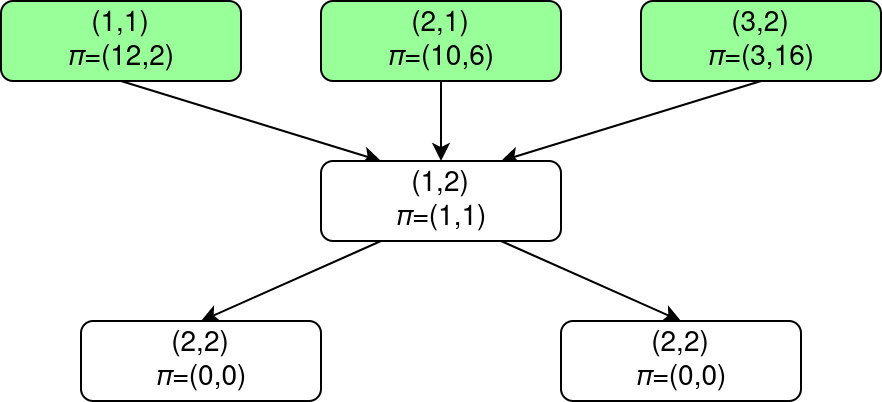
\includegraphics[height=6cm]{poset.jpeg}
    \caption{Partial ordering of the outcome set under Pareto dominance. Maximal elements marked in green.}
\end{figure}

\newpage
\section{Symmetric 3-player game}

\subsection{Filled-in matrix, Pareto optima}

Calculating all the numbers by hand would have been fairly error-prone, therefore I used a simple Python script to generate them. Adding a quick comparison to find Pareto-dominated outcomes was trivial. It simply compares every outcome with every other outcome, breaks the loop for each if it is dominated, prints the dominance relation and only selects those which aren't dominated.

\begin{figure}[h!]
    \centering
    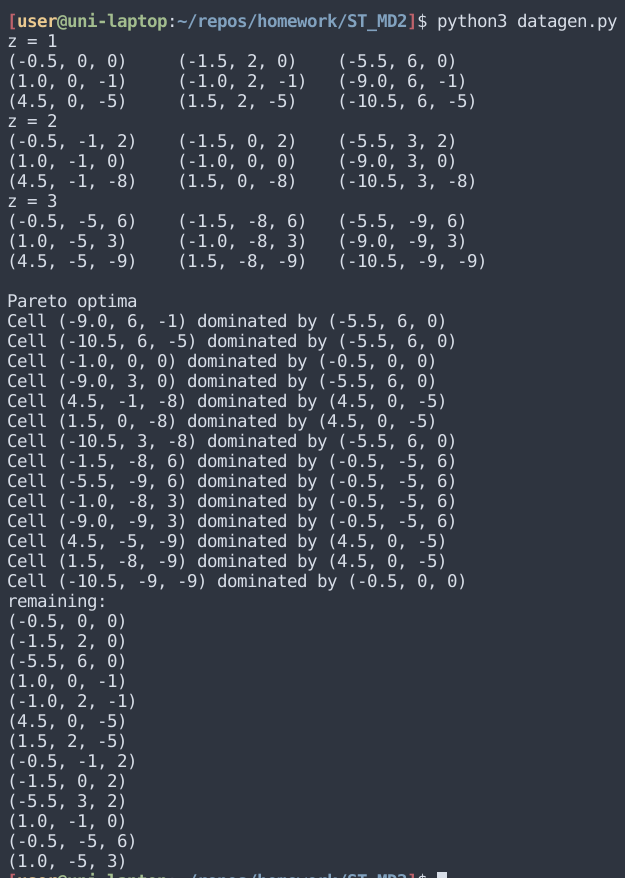
\includegraphics[height=14cm]{output.png}
    \caption{Payoff tensor, pareto optima.}
\end{figure}

\newpage
\subsection{Nash equilibrium}

In the general case, working out a Nash equilibrium for a 3x3x3 game could be a fairly involved process, but thankfully several simplifications are possible here.

First, notice that $\pi^1=f(x,y), \pi^2=g(y,z), \pi^3=h(z,x)$, which allows one to represent the entire payoff tensor with 3 matrices - one for each player (with rows being the value selected by this player)

\begin{equation}
    \boldsymbol{\pi_{xy}^1}=\begin{bmatrix}
        -\frac{1}{2} & -\frac{3}{2} & -\frac{11}{2} \\
        1 & -1 & -9 \\
        \frac{9}{2} & \frac{3}{2} & -\frac{21}{2} \\ 
    \end{bmatrix}
\end{equation}
\begin{equation}
    \boldsymbol{\pi_{yz}^2}=\begin{bmatrix}
        0 & 1 & -5 \\
        2 & 0 & -8 \\
        6 & 3 & -9 \\ 
    \end{bmatrix}
\end{equation}
\begin{equation}
    \boldsymbol{\pi_{zx}^3}=\begin{bmatrix}
        0 & 1 & -5 \\
        2 & 0 & -8 \\
        6 & 3 & -9 \\ 
    \end{bmatrix}
\end{equation}
The matrices of p2, p3 are also identical after this rotation.

The next key insight is that the middle row (2) of $\pi^2, \pi^3$ is dominated by mixed strategies with
\begin{equation}
    p(1)+(1-p)(3);\frac{1}{4} \leq p \leq \frac{2}{3}
\end{equation}
while the middle row (2) of $\pi^1$ is dominated by mixed strategies with
\begin{equation}
    p(1)+(1-p)(3);\frac{3}{10} \leq p \leq \frac{7}{10}
\end{equation}
allowing the middle row and column of every 3x3 matrix to be eliminated. 

The payoff matrices are thus

\begin{equation}
    \boldsymbol{\pi^1}=\begin{bmatrix}
        -\frac{1}{2} & -\frac{11}{2} \\
        \frac{9}{2} & -\frac{21}{2} \\ 
    \end{bmatrix},
    \boldsymbol{\pi^2}=\begin{bmatrix}
        0 & -5 \\
        6 & -9 \\ 
    \end{bmatrix},
    \boldsymbol{\pi^3}=\begin{bmatrix}
        0 & -5 \\
        6 & -9 \\ 
    \end{bmatrix}
\end{equation}
and by solving the resulting indifference equations
\begin{equation}
    p_x=p_z;0p_x-5(1-p_x)=6p_x-9(1-p_x)
\end{equation}
\begin{equation}
    -\frac{1}{2}p_y-\frac{11}{2}(1-p_y)=\frac{9}{2}p_y-\frac{21}{2}(1-p_y)
\end{equation}
we obtain
\begin{equation}
    p_x=p_z=\frac{2}{5};s_1=s_3=\frac{2}{5}(1)+\frac{3}{5}(3);E_2(eq.)=E_3(eq.)=-3
\end{equation}
\begin{equation}
    p_y=\frac{1}{2};s_2=\frac{1}{2}(1)+\frac{1}{2}(3);E_1(eq.)=-3
\end{equation}

As before, the players are all indifferent to the strategies within their mixed strategy support sets, but the fact that no player benefits by deviating can be verified by calculating the expected payoff of playing the remaining strategy

\begin{equation}
    E_1(2)=1*\frac{1}{2}-9*\frac{1}{2}=-4<E_1(eq.)
\end{equation}
\begin{equation}
    E_2(2)=E_3(2)=2*\frac{2}{5}-8*\frac{3}{5}=-4<E_2(eq.)=E_3(eq.)
\end{equation}


\end{document}